

\documentclass[12pt]{article} % article class, 12pt font

% load any packages you need for more custom stuff
\usepackage[margin=1in]{geometry} % set 1-inch margins
\usepackage{setspace}\doublespacing % set double spacing
\usepackage[superscript]{cite} % superscript numeric in-line citations
\usepackage{indentfirst} % indent the first paragraph of each section
\usepackage{graphicx} % enable displaying png format graphs
\usepackage{csvsimple} % enable importing tabular data
\usepackage{booktabs} % enable formulating tables
\usepackage{tabto} % allows you to tab stuff
% \newcommand\tab[1][1cm]{\hspace*{#1}}

% set title stuff
\title{Chutes and Ladders}
\newcommand{\authors}{Eli Sylvia-Lourde}
\author{Math 114 Mathematical Modeling\\St. Mary's College}
\date{March 22, 2019}

\begin{document}

% create title stuff
\hfill\authors % write the authors right-aligned
%\vspace{-0.5in} % reduce space before title
{\let\newpage\relax\maketitle} % print title

\section*{Problem Statement}
Hasbro,	the	manufacturer	of	the	board	game	Chutes	and	Ladders is	preparing	a	revision	of	the
game.	They	asked	you	do	make	some	estimates	of	the	playing	time.	From	their	own	in-house
testing	they	know	that	an	adult	takes	about	10	seconds	per	turn.	When	a	child	is	playing	with
an	adult,	a	child	typically	takes	15	seconds	per	turn.	When	children	are	playing	among
themselves,	they	take	about	25	seconds	per	turn.
Make	a	model	of	the	game	and	prepare	advice	for	Hasbro	on	what	they	should	say	about
playing	time	and	the	number	of	players	the	game	is	suitable	for.	Offer	advice	on	any	rule
changes	that	could	affect	the	playing	time.

\section*{Commentary}
In order to solve this problem, we are going to simulate how many turns it takes to play the game. Using this data, we will then simulate how many total turns it takes 2,4,6 people to play the game. We will then convert this to time based upon who is playing the game. Our answer will be an estimation of how long it takes adults, children and adults, and just children. Our final answer will be an equation that takes the number of adults and children playing the game and return how long it will take them to finish.

\section*{Modeling}
First we need to figure out how many rolls it takes, on average, to complete the game. Every player starts on square zero, rolls a d6, and then moves to the next square based upon what square they landed on. If the square that they are on + their roll is greater than 100, they stay where they are. If the sum = 100, they finish playing the game. Below is the code for modeling this:

\begin{verbatim}
def roll_d6():
    resp = randint(1, 6)
    return resp

# Index is where the square+roll is.
# square_dict[roll+square] = what square to end up after rolling
square_dict = [0,38, 2,3,14,5,6,7,8,31,10,11,12,13,14,15,6,17,18,
19,20,42,22,23,24,25,26,27,84,29,30,31,32,33,34,35,44,37,38,39,40,
41,42,43,44,45,46,26,48,11,50,67,52,53,54,55,53,57,58,59,60,61,19
,63,60,65,66,67,68,69,70,91,72,73,74,75,76,77,78,79,100,81,82,83,
84,85,86,24,88,89,90,91,92,73,94,75,96,97,78,99,100]

def chutes_and_ladders(roll, square):
    # If the player's roll goes beyond the board, nothing happens
    if (square + roll > 100):
        return square
    else:
        return square_dict[square+roll]

def play_game()
  square = 0
  rolls = 0
  roll_data = []
  number_of_games = 1000
  # Code that finds the average number of rolls to play the game
  while (square < 100 and len(roll_data) < number_of_games):
      rolls += 1
      roll = roll_d6()
      temp = square
      square = chutes_and_ladders(roll, square)
      # print("Started at {} rolled {}, went to {}".format(temp,roll,square))

      if (square == 100):
          roll_data.append(rolls)
          rolls = 0
          square = 0

    ave = 0
    for i in range(len(roll_data)):
        ave += roll_data[i]
    ave /= len(roll_data)
    print("Ave Rolls: {}".format(ave))
play_game()

\end{verbatim}

\section*{Data Analysis}
We can try to calculate a more accurate average by increasing the number of games that before finding the average game length. This results in the following graph:


% 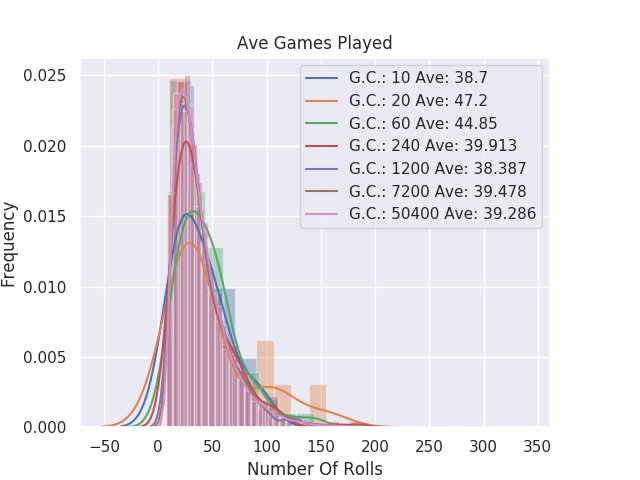
\includegraphics{Modeling.png}
noindent\makebox[\textwidth]{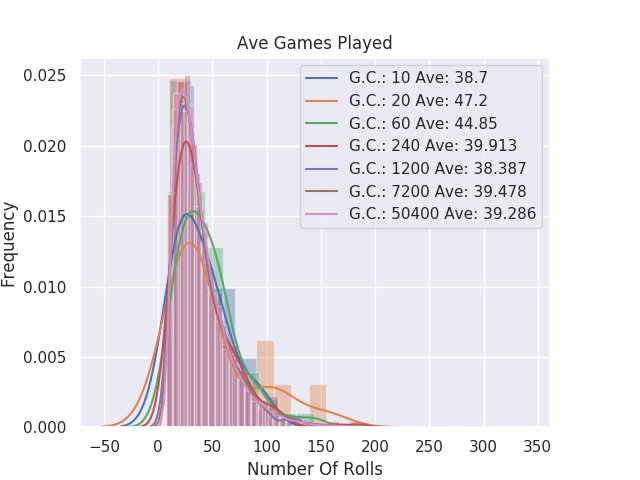
\includegraphics[width=\paperwidth]{Modeling.png}}
This model suggests that the average number of rolls it takes to finish a game is 39-40 rolls. Using this estimation, we can predict how long it takes one person to play a game.

\section*{When Play Time is Over}
Our model estimates that the average number of roles is 39. Using this, we can write the following equation to predict how long a game will take. $K_{n}=Number of Kids$ $A_{n}=Number of Adults$.
\\If there are adults:
\[Seconds = 39*10*A_{n} + 39*15*K_{n}\]
\\If there are no adults:
\[Seconds = 39*25*A_{n}\]

\section*{Changing Play Time}
A few things could be done to change the play time. If we wanted to increase the play time, we could decrease the magnitude of all ladders by 1 everytime someone landed on a ladder and increase the magnitude of all chutes by 1 everytime someone landed on a chute. We could flip this if we wanted to decrease the play time. For both examples, we would need to bound the chutes and ladders so that they could not go below 1 or above 100. If we wanted to increase the play time, we could allow people whose roll directs them to a position greater than 100 back to that position minus 100. This would result in them effectively restarting the game, which would certainly increase the play time. We could also move around where the chutes and ladders are positioned. If we wanted to make it very difficult to get beyond a certain square, we could put 5 chutes in a row, giving the player a 1 in 6 shot of making it through, depending how far away they were from the first chute. We could of course do the same thing with ladders if we wanted to make a particular section very easy.

As per usual, all of my code and such is on my github. This project is under Th3Lourde Mathematical Modeling Project 3 . If I messed the path to my project, I would of course be more than happy to provide the correct one. (Note the path provided is missing some underscores due to how latex handles them).

\end{document} % this ends your document
